\chapter{Silizium-PVD}
\label{appendix:silicon}

\section{Voruntersuchungen}

\begin{figure}
  \centering
  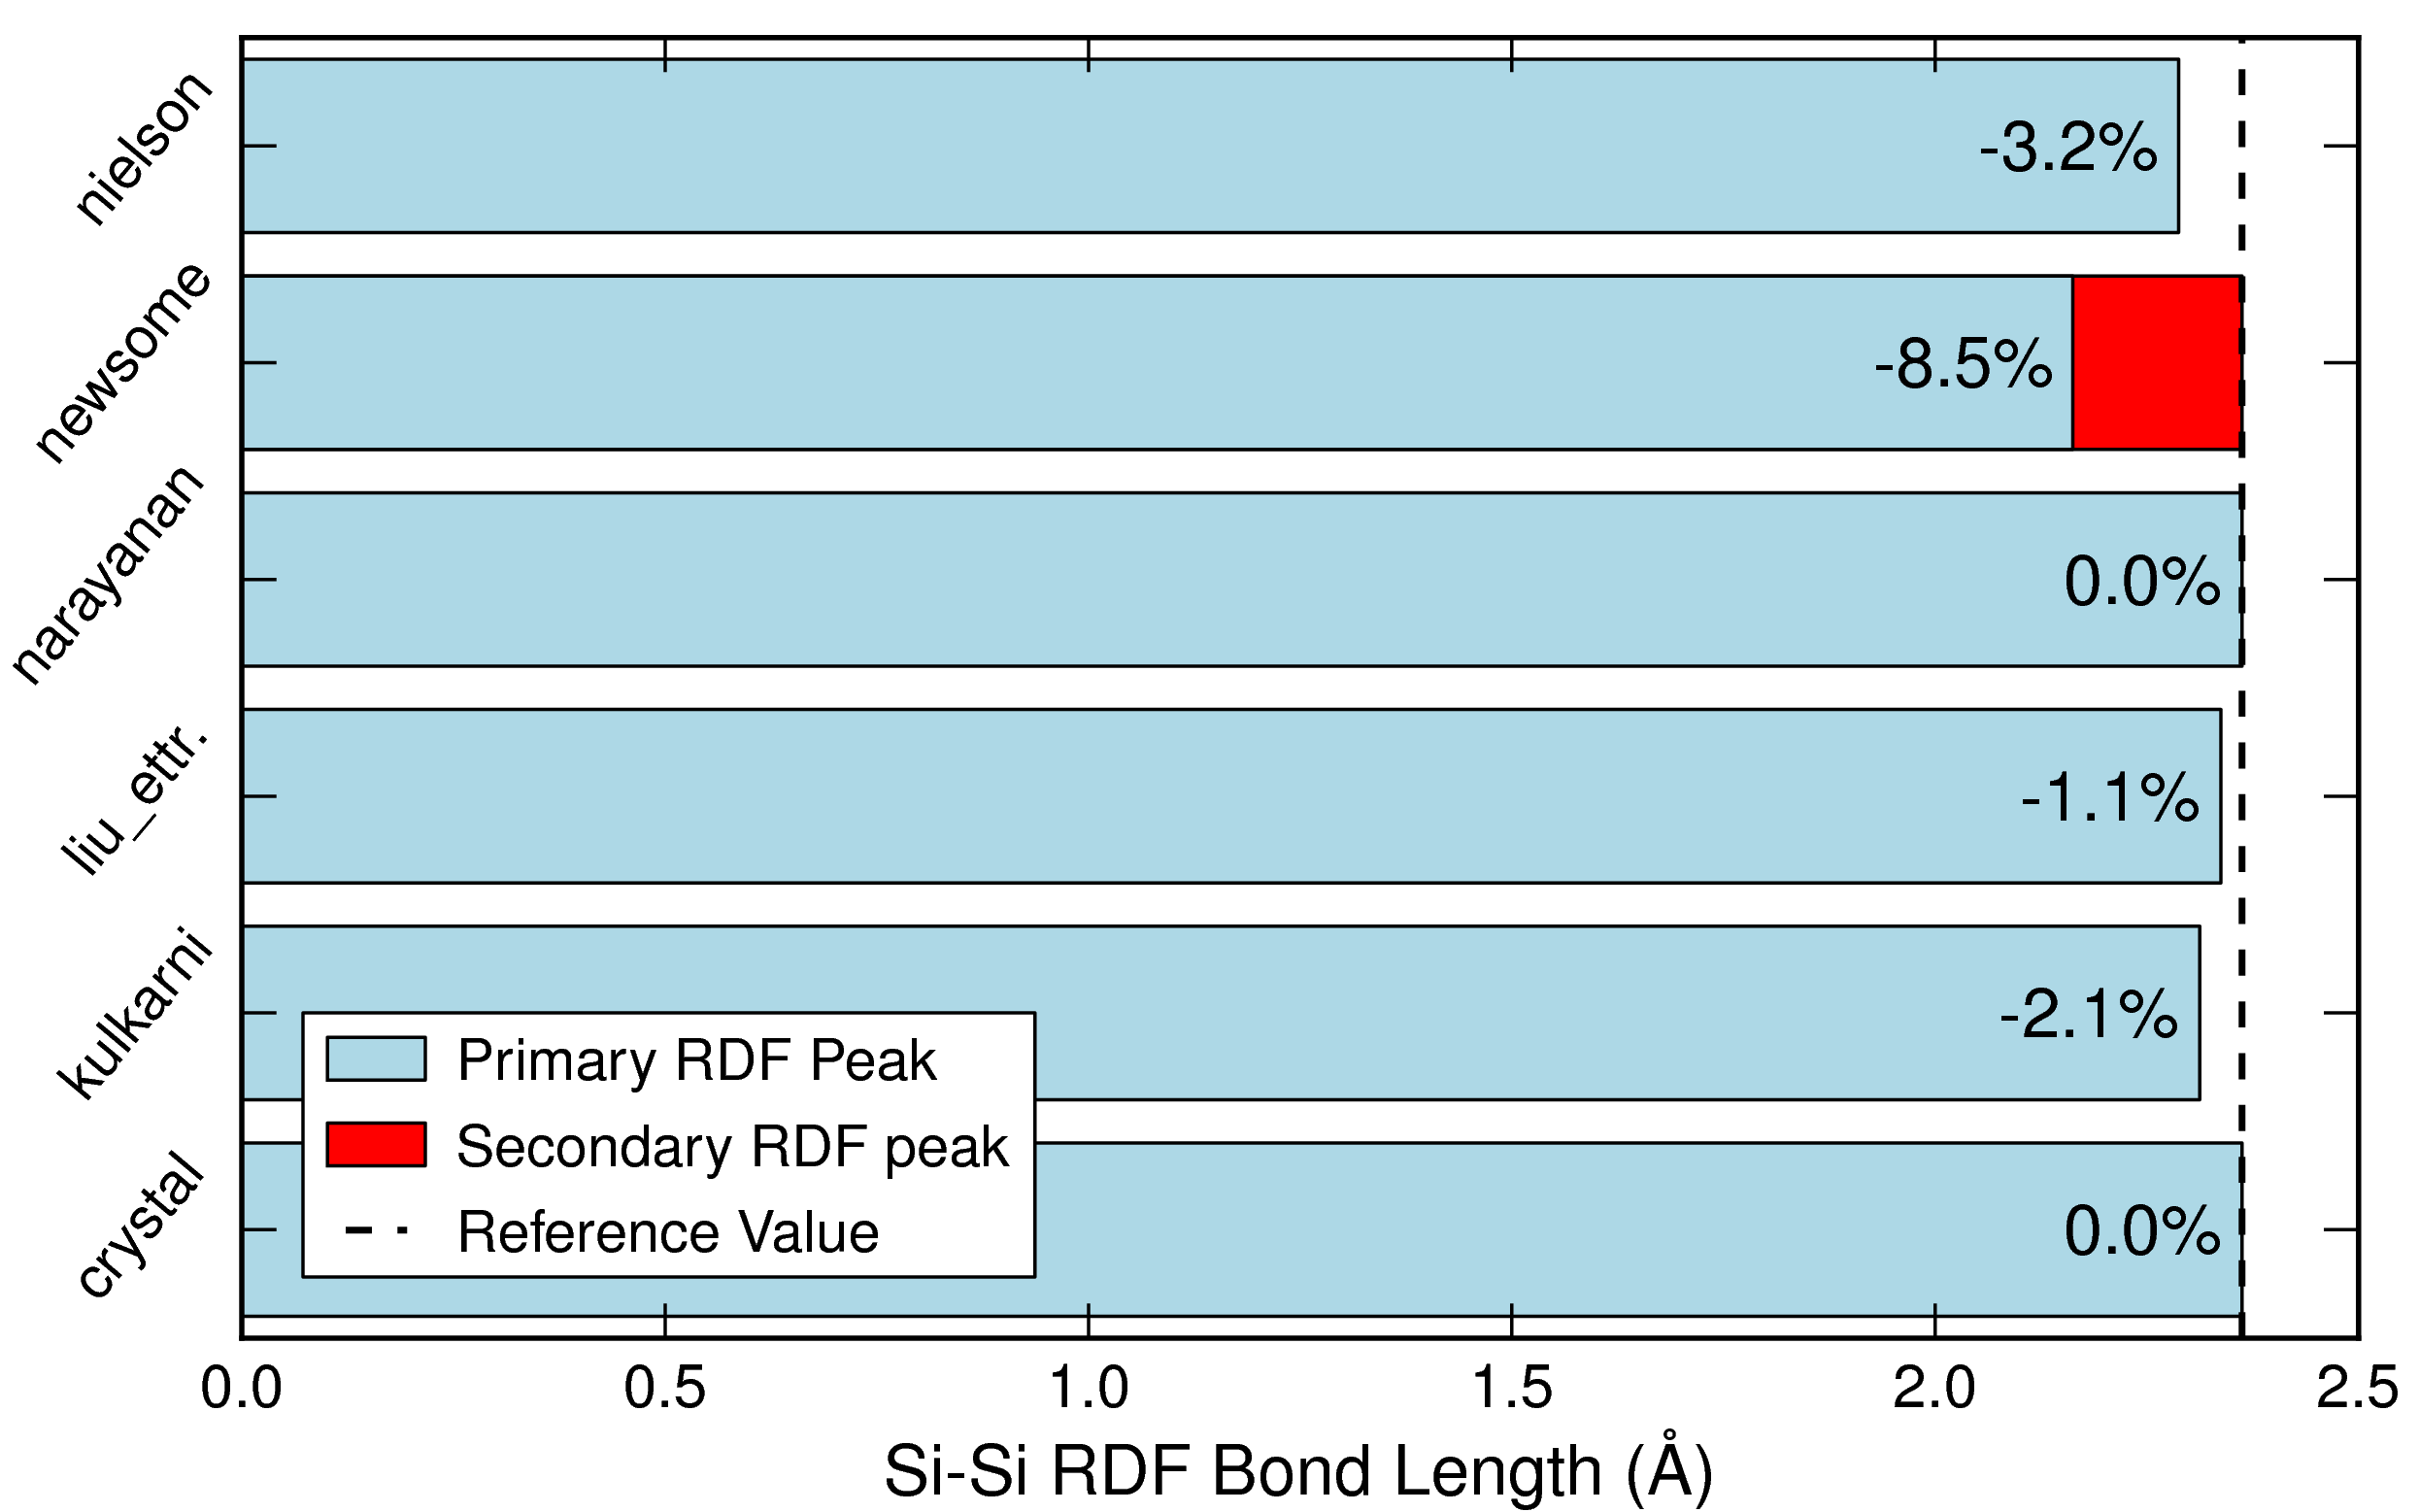
\includegraphics[width=10cm]{SiSi_npt_bondlengths}
  \caption[Bindungslängen von Kupfer im relaxierten Kristall für verschiedene Parametersätze]{Bindungslängen von Kupfer im relaxierten Kristall für verschiedene Parametersätze}
  \label{fig:sisibondlengths}
\end{figure}

\begin{figure}
  \centering
  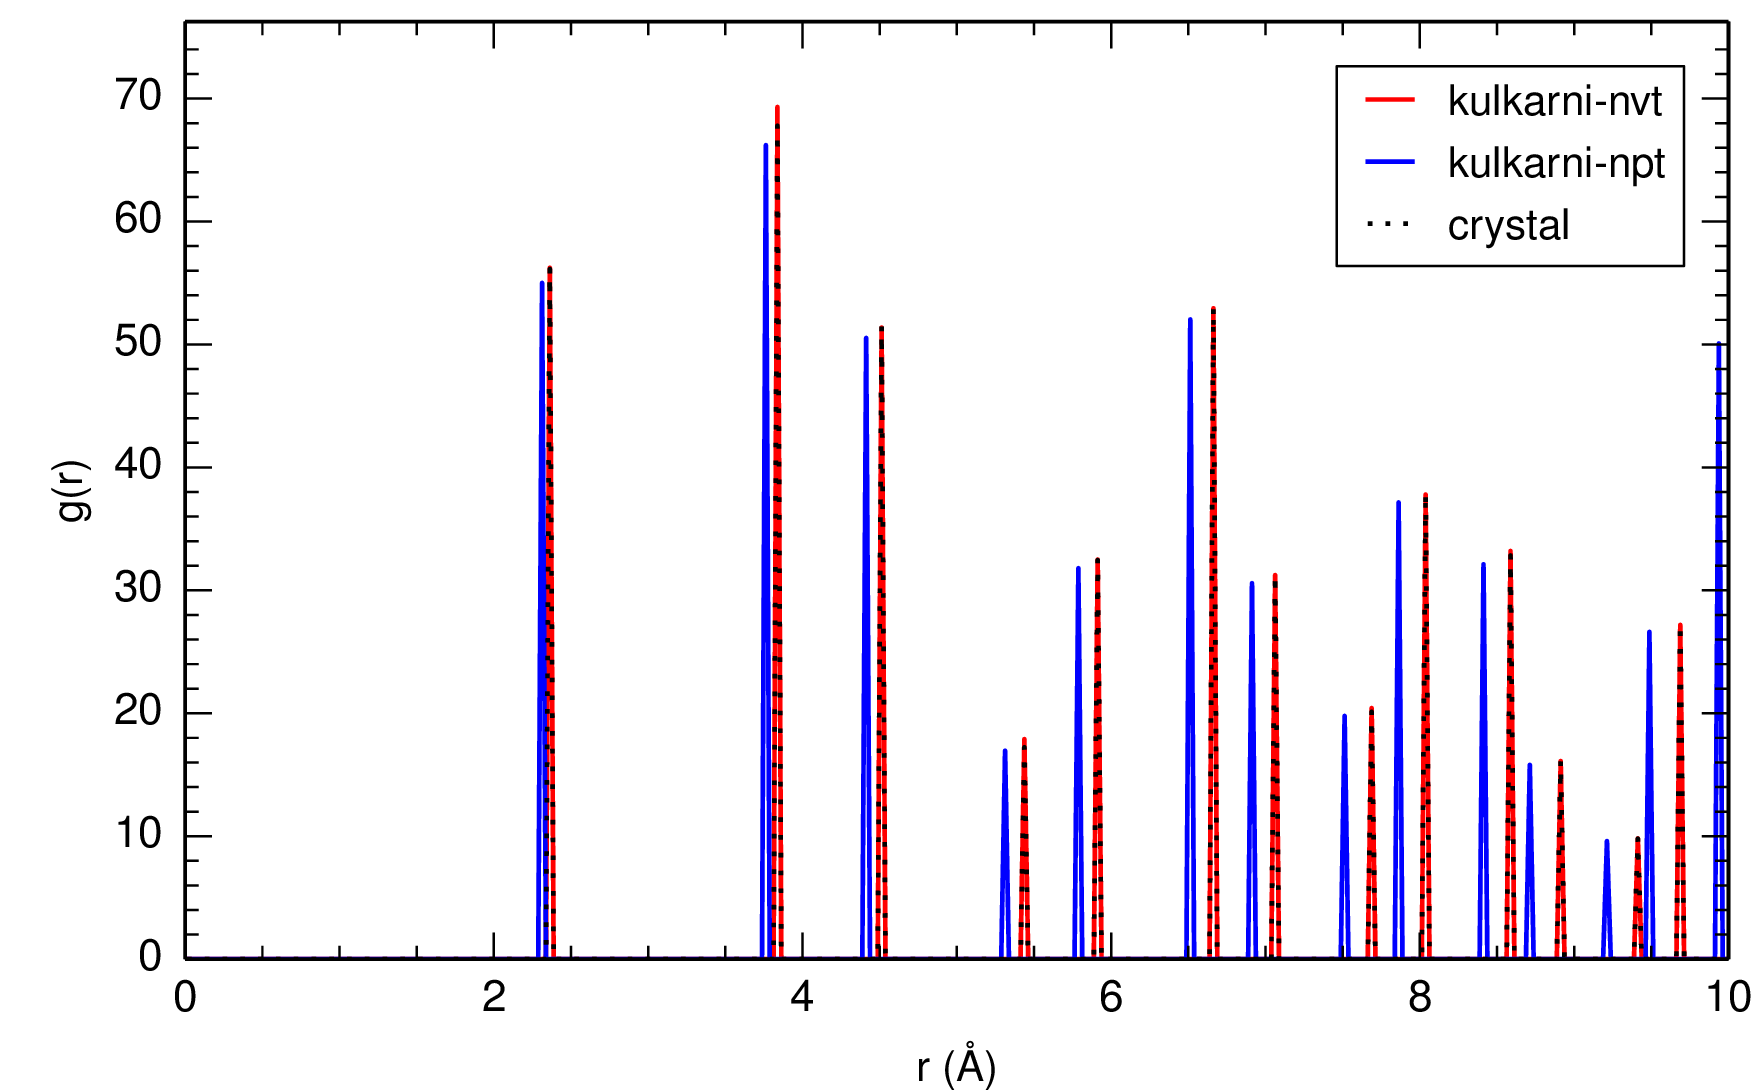
\includegraphics[width=10cm]{kulkarni_rdf_crystal}
  \caption[Radiale Verteilungsfunktion von kristallinem Silizium nach Relaxation mit Kulkarni-Parametersatz]{Radiale Verteilungsfunktion von kristallinem Silizium nach Relaxation mit Kulkarni-Parametersatz}
  \label{fig:kulkarnirdf}
\end{figure}

\begin{figure}
  \centering
  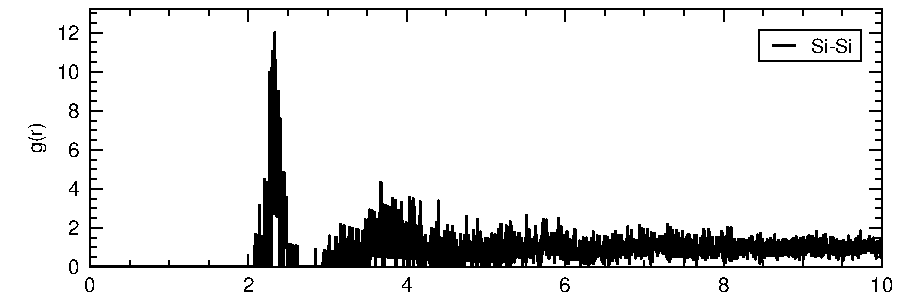
\includegraphics[width=\textwidth]{kulkarni_rdf_amorphous}
  \caption[Radiale Verteilungsfunktion von amorphem Silizium nach Relaxation mit Kulkarni-Parametersatz]{Radiale Verteilungsfunktion von amporphem Silizium nach Relaxation mit Kulkarni-Parametersatz}
  \label{fig:amorphousrdf}
\end{figure}

\begin{table}
  \begin{threeparttable}

    \caption[Vergleich der Eigenschaften amorpher Silizium-Materialien]{Vergleich der Eigenschaften amorpher Silizium-Materialien}
    \label{tab:amorphoussilicon}

    \oddrowcolors
    \begin{tabularx}{\textwidth}{|XXXX|}
      \hline
      \textbf{Parametrisierung} & \textbf{Bindungslänge} & \textbf{Koordinationszahl} & \textbf{Dichte}                          \\
      \hline
      (kristallin)              & \SI{2.352}{\angstrom}  & \num{4.00}                 & \SI{2.330}{\gpcc}                        \\
      (amorph)                  & ~                      & ~                          & \SI{2.3}{\gpcc}\cite{remes_optical_1998} \\
      Al\_Al0\_AlN              & \SI{2.379}{\angstrom}  & \num{4.59}                 & \SI{2.373}{\gpcc}                        \\
      kulkarni                  & \SI{2.339}{\angstrom}  & \num{4.05}                 & \SI{2.361}{\gpcc}                        \\
      liu\_ettr.                & \SI{2.401}{\angstrom}  & \num{4.10}                 & \SI{2.314}{\gpcc}                        \\
      narayanan                 & \SI{2.383}{\angstrom}  & \num{4.05}                 & \SI{2.365}{\gpcc}                        \\
      newsome                   & \SI{2.153}{\angstrom}  & \num{1.17}                 & \SI{2.398}{\gpcc}                        \\
      nielson                   & \SI{2.411}{\angstrom}  & \num{4.82}                 & \SI{2.358}{\gpcc}                        \\
      zhang                     & \SI{2.357}{\angstrom}  & \num{4.39}                 & \SI{2.329}{\gpcc}                        \\
      \hline                                                                                  
    \end{tabularx}

  \end{threeparttable}
\end{table}
